%  LaTeX support: latex@mdpi.com
%  In case you need support, please attach any log files that you could have, and specify the details of your LaTeX setup (which operating system and LaTeX version / tools you are using).

%=================================================================

% LaTeX Class File and Rendering Mode (choose one)
% You will need to save the "mdpi.cls" and "mdpi.bst" files into the same folder as this template file.

%=================================================================

\documentclass[remotesensing,article,accept,moreauthors,pdftex,12pt,a4paper]{mdpi} 
%--------------------
% Class Options:
%--------------------
% journal
%----------
% Choose between the following MDPI journals:
% actuators, administrativesciences, aerospace, agriculture, agronomy, algorithms, animals, antibiotics, antibodies, antioxidants, appliedsciences, arts, atmosphere, atoms, axioms, behavioralsciences, bioengineering, biology, biomedicines, biomolecules, biosensors, brainsciences, buildings, cancers, catalysts, cells, challenges, chemosensors, children, chromatography, climate, coatings, computation, computers, cosmetics, crystals, dentistryjournal, diagnostics, diseases, diversity, econometrics, economies, education, electronics, energies, entropy, environmentalsciences, environments, fibers, foods, forests, futureinternet, galaxies, games, genes, geosciences, healthcare, humanities, informatics, information, inorganics, insects, ijerph, ijfs, ijms, ijgi, jcdd, jcm, jdb, jfb, joi, jlpea, jmse, jpcg, jpm, jrfm, jsan, land, laws, life, lubricants, machines, marinedrugs, materials, mathematics, medicalsciences, membranes, metabolites, metals, microarrays, micromachines, microorganisms, minerals, molbank, molecules, nanomaterials, ncrna, nutrients, pathogens, pharmaceuticals, pharmaceutics, pharmacy, photonics, plants, polymers, processes, proteomes, publications, religions, remotesensing, resources, risks, robotics, sensors, socialsciences, societies, sports, sustainability, symmetry, systems, technologies, toxics, toxins, vaccines, veterinarysciences, viruses, water
%---------
% article
%---------
% The default type of manuscript is article, but could be replaced by using one of the class options: 
% article, review, communication, commentary, bookreview, correction, addendum, editorial, changes, supfile, casereport, comment, conceptpaper, conferencereport, meetingreport, discussion, essay, letter, newbookreceived, opinion, projectreport, reply, retraction, shortnote, technicalnote, creative
%----------
% submit
%----------
% The class option "submit" will be changed to "accept" by the Editorial Office when the paper is accepted. This will only make changes to the frontpage (e.g. the logo of the journal will get visible), the headings, and the copyright information. Journal info and pagination for accepted papers will also be assigned by the Editorial Office.
% Please insert a blank line is before and after all equation and eqnarray environments to ensure proper line numbering when option submit is chosen
%------------------
% moreauthors
%------------------
% If there is only one author the class option oneauthor should be used. Otherwise use the class option moreauthors.
%---------
% pdftex
%---------
% The option "pdftex" is for use with pdfLaTeX only. If eps figure are used, use the optioin "dvipdfm", with LaTeX and dvi2pdf only.

%=================================================================
\setcounter{page}{1}
\lastpage{x}
\doinum{10.3390/------}
\pubvolume{xx}
\pubyear{2014}
\history{Received: xx / Accepted: xx / Published: xx}
%------------------------------------------------------------------
% The following line should be uncommented if the LaTeX file is uploaded to arXiv.org
%\pdfoutput=1

%=================================================================

% Add packages and commands to include here
% The amsmath, amsthm, amssymb, hyperref, caption, float and color packages are loaded by the MDPI class.
%\usepackage{graphicx}
%\usepackage{subfigure,psfig}


\usepackage{xcolor}
\usepackage{graphicx}
\usepackage{subcaption} 
\usepackage{url}
\usepackage{multirow}
\usepackage{amsmath}
\usepackage{amssymb}
\usepackage{rotating}

\newcommand\red[1]{\textcolor{red}{#1}} % Red marker to declare errors.

%=================================================================
%% Please use the following mathematics environments:
%\theoremstyle{mdpi}
%\newcounter{thm}
%\setcounter{thm}{0}
%\newcounter{ex}
%\setcounter{ex}{0}
%\newcounter{re}
%\setcounter{re}{0}
%\newtheorem{Theorem}[thm]{Theorem}
%\newtheorem{Lemma}[thm]{Lemma}
%\newtheorem{Characterization}[thm]{Characterization}
%\newtheorem{Proposition}[thm]{Proposition}
%\newtheorem{Property}[thm]{Property}
%\newtheorem{Problem}[thm]{Problem}
%\newtheorem{Example}[ex]{Example}
%\newtheorem{Remark}[re]{Remark}
%\newtheorem{Corollary}[thm]{Corollary}
%\newtheorem{Definition}[thm]{Definition}
%% For proofs, please use the proof environment (the amsthm package is loaded by the MDPI class).

%=================================================================

% Full title of the paper (Capitalized)
\Title{Hyperspectral Classification of Savanah Tree Species Using $k$-fold Cross-Validated Non-linear Support Vector Machines }

% Authors (Add full first names)
\Author{Morteza Shahriari Nia $^{1,}$*, Daisy Zhe Wang $^{1}$, Milenko Petrovic $^{2}$, Stephanie Ann Bohlman $^{3}$ and Paul Gader $^{1}$}

% Affiliations / Addresses (Add [1] after \address if there is only one affiliation.)
\address{%
$^{1}$ Department of Computer and Information Science and Engineering, University of Florida, 432 Newell Dr., Gainesville, Florida 32611, USA\\
$^{2}$ Institute for Human and Machine Cognition, 15 SE Osceola Ave, Ocala, Florida 34471, USA\\
$^{3}$ School of Forest Resources and
Conservation, 349 Newins Ziegler Hall, Gainesville, Florida
32611, USA}

% Contact information of the corresponding author (Add [2] after \corres if there are more than one corresponding author.)
\corres{msnia@cise.ufl.edu}

% Abstract (Do not use inserted blank lines, i.e. \\) 
\abstract{Identifiying savannah species at ecological scale is major mile-stone in measuring biomass, carbon reserves, drought and invasive specie spread predictions. In this paper we perform classification and geo-mapping of tree species from hyperspectral imagery collected using AVRIS airborne sensors and atmospherically corrected using ATCOR. This study classifies four common savannah tree species in Ordway-Swisher Biological Station in north-central Florida, USA. Among predictors we found NDVI, the NIR wavelngths (0.73$\mu m$) and removal of water absorption bands (1.36$\mu m$ - 1.44$\mu m$) and (1.8$\mu m$ - 1.96$\mu m$) to be most useful. Gaussian filter was used to avoid sensor measurements and calibration errors in reflectance data. We employed various classification techniques out of which Support Vector Machines with a third degree polynomial kernel outperformed others. Our classification scheme produces accurate predictions of 80.02\% at pixel level. We also evaluated the performance of FLAASH and ATCOR atmospheric corrections on prediction accuracy. This research was performed as a pilot study for the National Ecological Observatory Network-Airborne Observation Platform protocols.}

% Keywords: add 3 to 10 keywords
\keyword{Specie classification; Hyperspectral; Savannah; Support Vector Machines; Ordway-Swisher Biological Station; High spatial and spectral resolution; Pixel-level classification; National Ecological Observatory Network; Airborne Observation Platform protocols; NEON-AOP}

% The fields PACS, MSC, and JEL may be left empty or commented out if not applicable
%\PACS{}
%\MSC{}
%\JEL{}

\begin{document}

\section{Introduction}

Mapping tree species by remote sensing techniques is an essential step in understanding how species play roles in ecological scale. This will enable us to study land covers, climate change, invasive specie changes, plant competitions, predict fire potentials and spreading routes, soil characteristics and etc \cite{scholes1997tree, colgan2012mapping}. This kind of work has only been possible via the technological advancements in hyperspectral imagey. 

Various studies have dealt with identifying tree species at both pixel level and crown level. Carnegie Airborne Observatory\footnote{http://cao.stanford.edu/} (CAO)  is a major prioneer in employing airborne technology for remote sensing of ecology. Here we briefly overview some of their works as well as other research groups contributions. Colgan et al. \cite{colgan2012mapping} uses a two stage Support Vector Machines (SVM) at pixel level and at crown level for tree specie classification; LiDAR data is used for crown segmentation. F\'{e}ret and Asner \cite{feret2013tree} study the accuracy of various parametric/non-parametric supervised classification techniques and observed that there is a clear advantage in using regularized discriminant analysis, linear discriminant analysis, and support vector machines among others. There are other schools of thought that use unsupervised techniques. For example Baldeck and Asner \cite{baldeck2013estimating} try to measure how similar beta diversity of regions are; they use distance measures such as Euclidean distance and K-means clustering. Using these clustering techniques one can have a quick understanding of beta diversities and avoid costly and time consuming field data collections. This line of research needs more work as about 50\% of pixels are classified as \textit{other}, therefore any conclusion at this scale of uncertainty is not necessarily helpful, the same holds for \cite{baldeck2014landscape}.

Cho et al. \cite{cho2012mapping} compares accuracies when different hyperspectral sensors of CAO, WorldView2 and QuickBird are utilized by convolving the 72 bands of CAO to eight and four multispectral channels available in the WorldView-2 and Quickbird satellite sensors, respectively. Interestingly enough they observed that WorldView-2 produced more accurate classification results then QuickBird and finally CAO. Clark et a. take on another perspective and compare lab measurements to pixel and to crown level \cite{clark2005hyperspectral} and try to identify important wavelength regions for specie discrimination. They observed that optimal regions of the spectrum for species discrimination varied with scale. However, near-infrared (700-1327$nm$) bands were consistently important regions across all scales. Bands in the visible region (437-700$nm$) and shortwave infrared (1994-2435$nm$) were more important at pixel and crown scales  \cite{clark2005hyperspectral}. Clark et al.  in another work evaluates the effects of differnet metrics used for classification (indexes, derivatives, signals themselves and all together) \cite{clark2012species}. There are other tree specie classification works such as \cite{dalponte2014tree, feret2012semi, feret2013tree, ghosh2014framework, immitzer2012tree, naidoo2012classification, ustin2009retrieval} that share the same aproach with minor variations. 

Sometimes specially tailored tools and methodologies in this field are necessary. As an example, one should note that differnet bands in a hyperspectral image have differnet signal to noise ratios, and Principal Components (PC) transform will not always result in components with a steadily increasing noise level. This makes setting a cut-off point difficult. Minimum Noise Fraction (MNF)   \cite{green1988transformation} is a modified PC transform which produces a set of principal component images ordered in terms of decreasing signal quality. 


National Ecological Observatory Network (NEON) is a long term ecology monitoring project for for discovering, understanding and forecasting the impacts of climate change, land use change, and invasive species at continental-scale. NEON, funded by National Science Foundation (NSF) in the US, will operate for 30 years starting 2016. Local ecological measurements at sites distributed within 20 ecoclimatic domains across the contiguous United States, Alaska, Hawaii, and Puerto Rico will be coordinated with high resolution, regional airborne remote sensing observations \cite{kampe2010neon}. Twenty terrestrial wildland core sites statistically represent unmanaged wildland conditions across the U.S. for NEON's 30-year lifetime. NEON moves an additional 40 relocatable terrestrial sites every five to seven years to locations where they may best capture specific ecological phenomena such as land use change and regional nitrogen deposition. Thirty-six aquatic sites collect representative aquatic data. Many aquatic sites are located near core and relocatable terrestrial sites\footnote{http://www.neoninc.org/science/domains\#sthash.aW1THj1N.dpuf}.Airborne Observation Platform (AOP) would be the remote sensing platform with equipments of meter/sub-meter resolution for hyperspectral and Light Detection and Ranging (LiDAR) measurements. This paper is a pilot study on the pre-mission airborne hyperspectral data collected. No operation at the scale and time span of NEON has been ever carried out before and a thorough study of the opportunities and challenges ahead is necessary specifically in the \textit{remote sensing} perspective where the volume of data can quickly become overwhelming \cite{neon2010aopdatarelease}.

\section{Data Collection}

The NEON Southeast Domain 3 contains the southern portions of the Gulf Coast states, half of South Carolina, and all of Florida except for the southern tip. The candidate core site for Domain 3 is located at the Ordway-Swisher Biological Station (OSBS) which is a 37-square kilometer area in Putnam County in north-central Florida and is managed jointly by the University of Florida and the Nature Conservancy\footnote{http://ordway-swisher.ufl.edu/index.htm} with UTM coordinates: 3,285,000 Northing, 405,000 Easting and UTM Zone 17. OSBS features diverse natural forests, small pine plantations nearby, a range of wildlife species that reflects the area's ecological communities, and a 75-year history of low human impact.  Nine major plant communities exist within the region as defined by the Florida Natural Areas Inventory and these diverse targets are populated by sandhill, xeric hammock, upland mixed forest, baygalls, basin swamp, basin marsh, marsh lake, clastic upland lake and sandhill upland lakes. The sandhills community is managed using prescribed burning on a scheduled 3-year rotation. The ground sampling part of this campaign focused on a sandhill ecosystem dominated by Long-Leaf Pine (\textit{Pinus Palustris}) and Turkey Oak (\textit{Quercus Laevis}). The sandhill ecosystem at OSBS was selected for concurrent ground measurements because a NEON instrumented tower will be located within this ecosystem type \cite{neon2010aopdatarelease, kampea2010aop}.

Since the instrumentation slated for deployment on the eventual AOP remote sensing payloads were not yet available, airborne spectroscopic and LiDAR measurements were made during this campaign using existing systems that exhibit similar performance characteristics as the instrumentation under development \cite{kampea2010aop}.

Hyperspectral: AVIRIS (Airborne Visible/Infrared Imaging Spectrometer) operated by personnel from the Jet Propulsion Laboratory (JPL) deployed on a Twin Otter DeHavilland DHC-6-300 aircraft in partnership with the National Aeronautics and Space Administration Terrestrial Ecology Program was used to collect data. JPL has flown on two separate days over OSBS: morning of September 4, 2010 (between 9:30 and 10:30 am) and mid-day of September 10, 2010. Both of the flights were flown at approximately 4000m AGL at approximately 90 knots on a Twin Otter aircraft with zenith angle of 180.0 and azimuth angle of 0.0. Details of these flights can be seen in Figure \ref{fig:hyperspectral}. Dependent on flight line, pixel size ranges from 3.3m to 3.6m. Hyperspectral data was atmospherically corrected using FLAASH \cite{adler1998flaash} and ATCOR \cite{richter2005atmospheric} algorithms. There are 8 flight lines and the total size of compressed data is 33GB. There are 224 bands recorded, with wavelengths from 365.93 nm to 2496.24 nm. 
%Concurrent ground data includes weather parameters, aerosol optical depth, field spectra of various canopies, and Leaf Area Index (LAI) measurements.

Atmospheric characterization relied on measurements of a CIMEL sun photometer in coordination with the NASA Aerosol Robotic Network\footnote{NASA AERONET: http://gcmd.nasa.gov/records/GCMD\_AERONET\_NASA.html}. Measurements were collected on September 4, 2010 and the the derived atmospheric information was used to improve the atmospheric correction of the AVIRIS spectrometer data. You can find the detailed measurements such as aerosol optical thickness, water vapor, and etc online\footnote{http://aeronet.gsfc.nasa.gov/cgi-bin/type\_one\_station\_opera\_v2\_new?site=Ordway-Swisher}.
 



% http://tex.stackexchange.com/questions/42968/reduction-of-space-between-two-sub-figures
\begin{figure}[tp]
  % Fixed length
  \centering
  \subcaptionbox{Flights ground tracks\label{fig3:gaussian smoothing:a}}{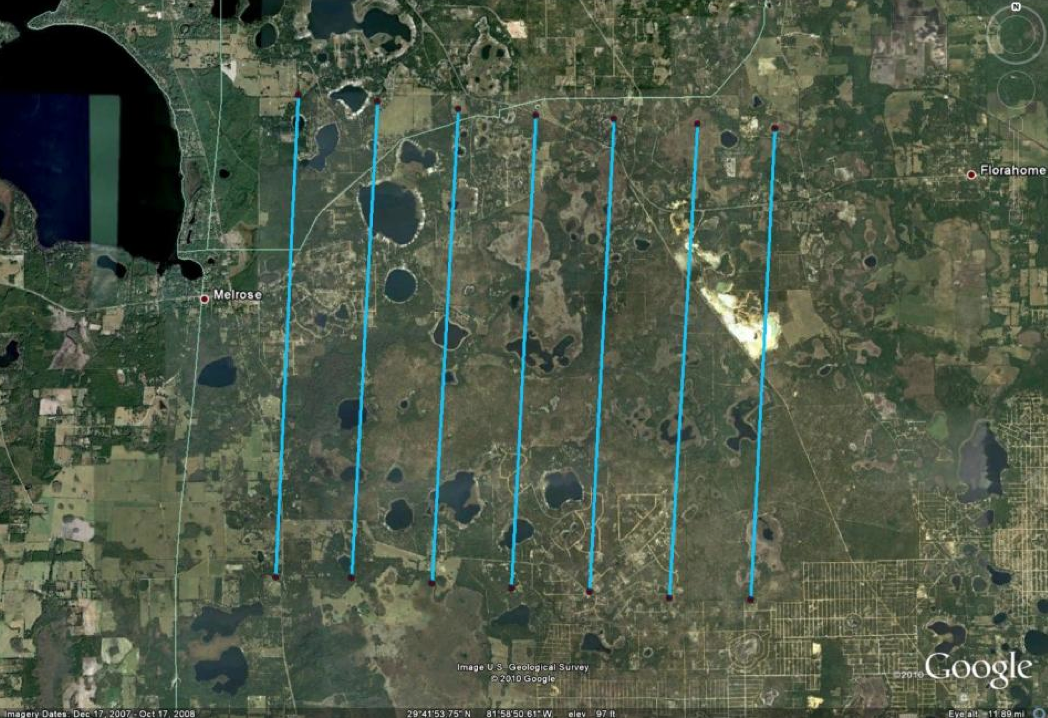
\includegraphics[height=1.7in,keepaspectratio]{./images/JPL_AVIRIS_flight_ground_tracks_OSBS_9_4_10.png}}\hspace{1em}%
  \subcaptionbox{Hyperspectral true-color mosaic, morning 09/04/2010\label{fig3:gaussian smoothing:a}}{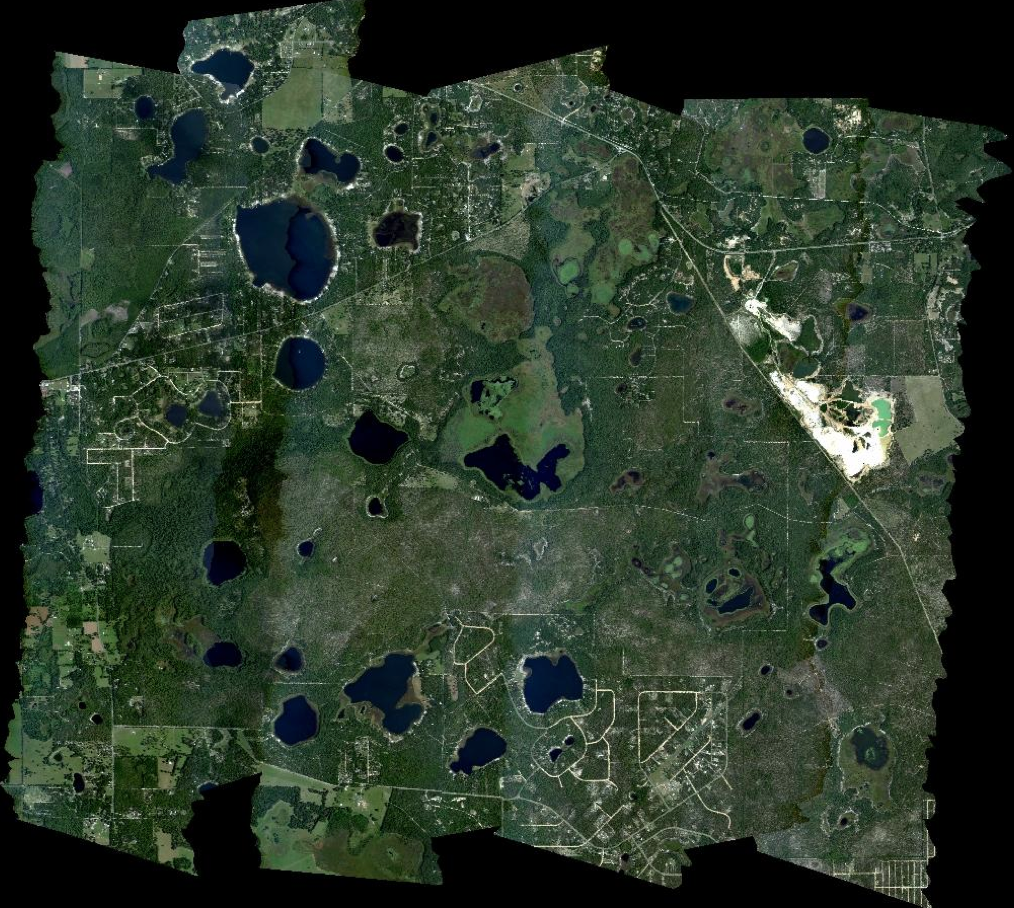
\includegraphics[height=1.7in,keepaspectratio]{./images/JPL_AVIRIS_true_color_mosaic_OSBS_9_4_10.png}}\hspace{1em}%
  \subcaptionbox{Hyperspectral true-color mosaic, mid-day 09/10/2010\label{fig3:gaussian smoothing:b}}{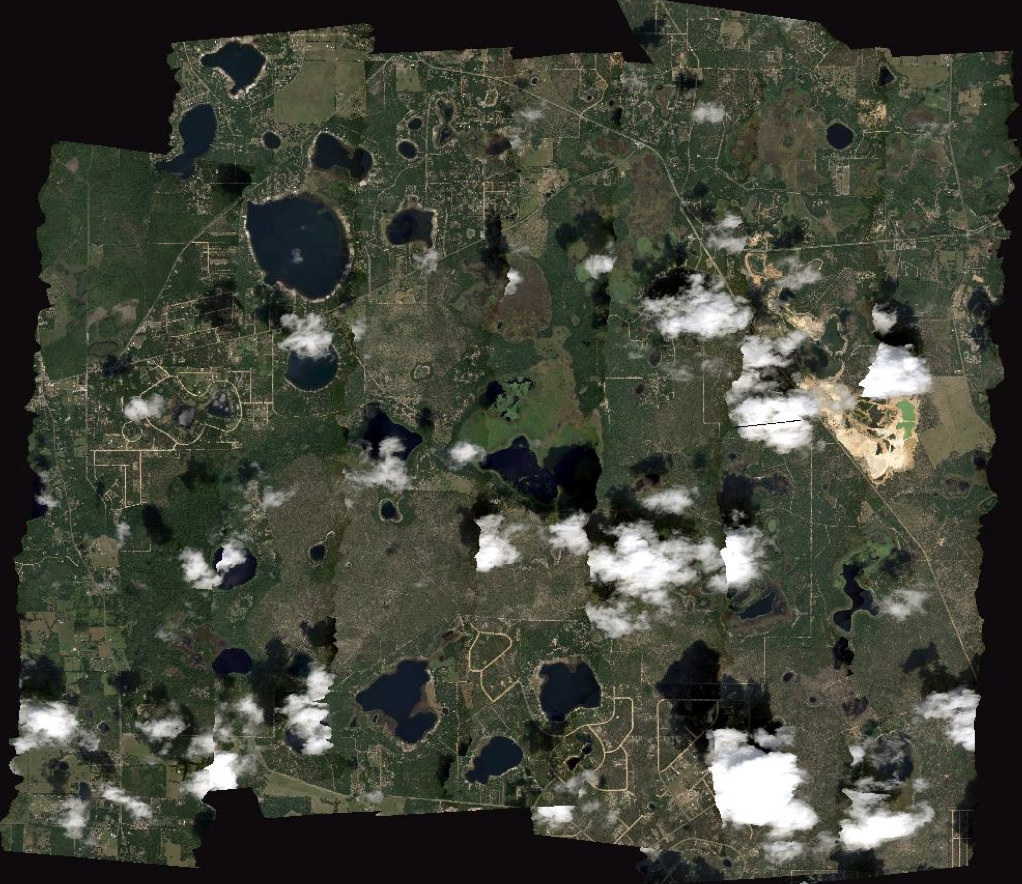
\includegraphics[height=1.7in,keepaspectratio]{./images/JPL_AVIRIS_true_color_mosaic_OSBS_9_10_10.png}}
   \caption{JPL AVRIS flights over OSBS \cite{neon2010aopdatarelease}}
 \label{fig:hyperspectral}
\end{figure}








LiDAR: The National Center for Airborne Laser Mapping (NCALM)\footnote{http://www.ncalm.cive.uh.edu/} coordinated the waveform-LiDAR flights in the same study areas and as  with the AVIRIS flights \cite{neon2010aopdatarelease}. As shown in Figure \ref{fig:lidar}, NCALM flew an Optech Gemini\footnote{Optech Gemini LiDAR sensor: http://www.optech.ca/gemini.htm} waveform-LiDAR with a nominal altitude flight covering the entire OSBS on September 1, 2010. In total there were 33 flight lines collected over OSBS both in the morning and in the afternoon, 7 flight lines were re-flown due to clouds. Range scale of LiDAR data was at 1.0m and up to five returns were recorded. The parameters for the data collected are 70 kHz PRF, wide beam divergence of 0.8 mrad, 20 deg half scan angle, and 40 Hz scan frequency. The GPS/IMU navigation data are processed using the Applanix POSPac MMS software to determine the position, orientation, and trajectory of the aircraft. The discrete LiDAR return data are processed using the Optech DASHMap software to create point cloud data files in ASPRS LAS 1.2 format \cite{las12format}. Each point data record contains information such as the intensity for the laser pulse and the X, Y, and Z geolocation of the point return. DASHMap reports up to four discrete returns: first, second, third, last. Using the geolocation information, the point clouds can be visualized 3-dimensionally.


% http://tex.stackexchange.com/questions/42968/reduction-of-space-between-two-sub-figures
\begin{figure}[tp]
  % Fixed length
  \centering
  \subcaptionbox{Flights ground tracks\label{fig3:gaussian smoothing:a}}{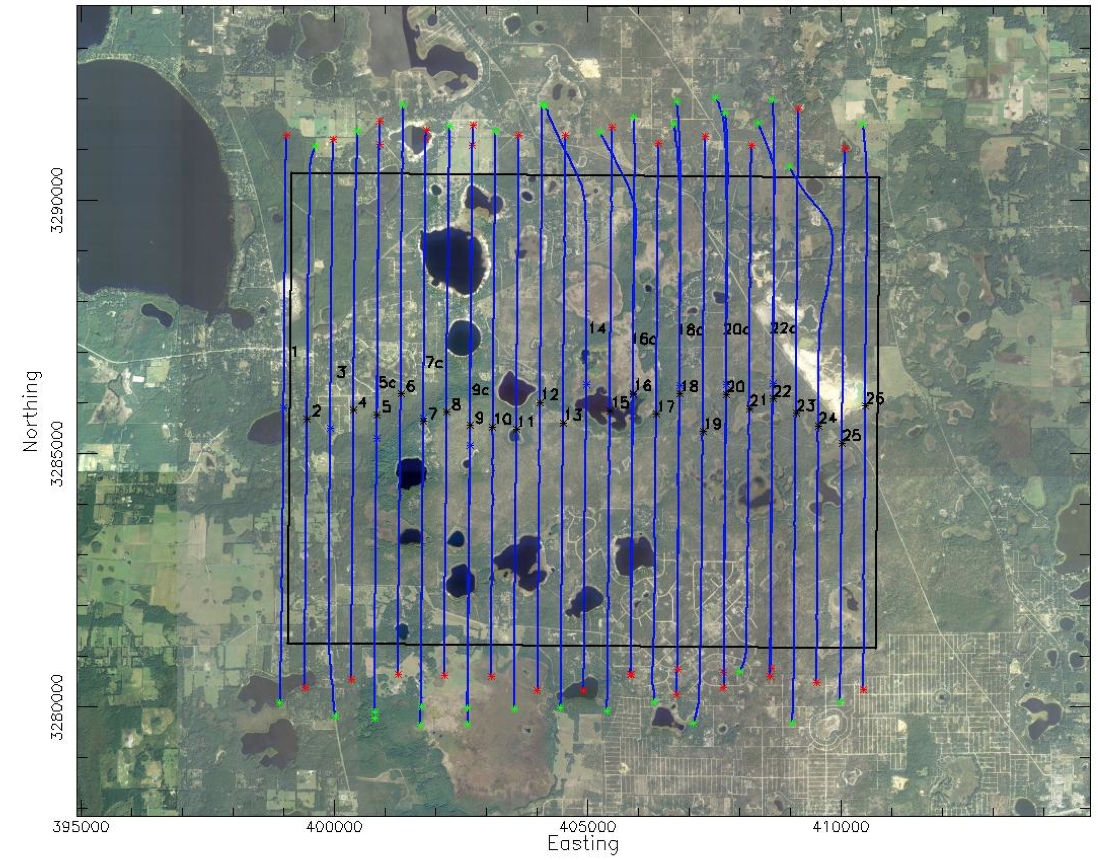
\includegraphics[height=2.3in,keepaspectratio]{./images/NCALM_flight_ground_tracks_OSBS_9_01_10.png}}\hspace{3em}%
  \subcaptionbox{LiDAR color height mosaic\label{fig3:gaussian smoothing:b}}{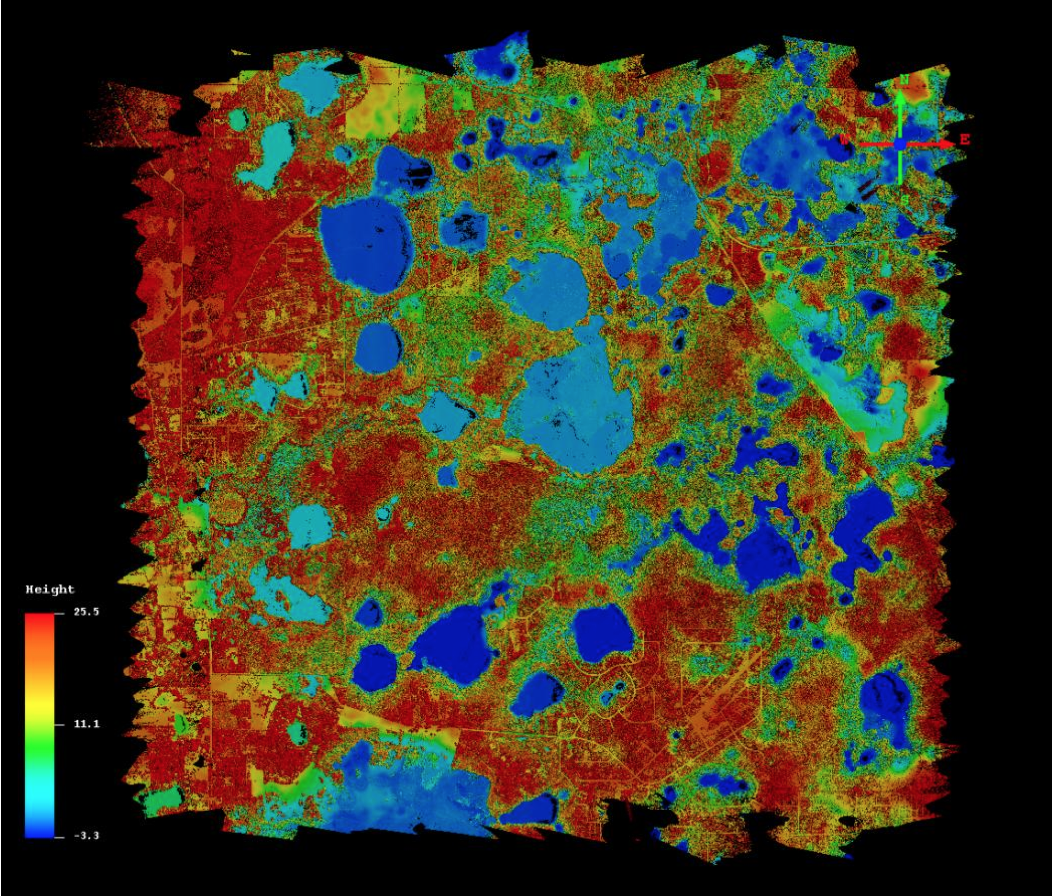
\includegraphics[height=2.3in,keepaspectratio]{./images/NCALM_Optech_Gemini_LiDAR_color_height_mosaic_OSBS_9_01_10.png}}
   \caption{NCALM Optech Gemini LiDAR flights over OSBS 09/01/2010 \cite{neon2010aopdatarelease}}
 \label{fig:lidar}
\end{figure}



\section{Specie Classification}

Upon the collection, orthorectification and atmospheric correction of hyperspectral and LiDAR data we work on identifying tree species. With the resolution of images being about 3 meters we are not getting pure pine or oak signlas and there is lots of mixing going on. A pixel's hyperspectral values is a linear/nonlinear mixing of leaf, branch, soil, shade, and other signals. The timing of fights (September) adds to the challenge: leafs might not be as green or that some trees might have already started to lose leaves and this leads to us getting more branch signals. Further more Longleaf pine is a conifer (needlelaf), unlike broadleaf trees where signal return can be more accurate. 

\subsection{Field Data}


For our classification task, we collected ground data of identifying tree species on February 28th, 2014. We drove to OSBS with a laptop that has ArcMap installed on and the ENVI image loaded in it, we connected a professional grade GPS to the laptop. ArcMap read GPS coordniates and mapped the polygons in the ENVI image. In this way, we marked several geo-polygons that had uniform plant species in the ENVI image. Later on we overlayed the identified polygons with proper JPL AVRIS flight which had the least amout of clouds. In this case we bookmarked flight \#4 on morning of 09/04/2010. This approach works pretty accurate if you are not in a dense forest such as tropical forests where GPS signal under the tree canopy has high deviations due to NLOS (no-line of sight) of GPS signals. Even with these considerations GPS still doesn't work that great and you need to mark several items such as by this road, close to this big tree to be able to later on mark your points in the map and avoid shifts in coordinats.

Alltogether we identified species for 452 pixels. In Table \ref{table:field data} you can fidn the details of identified Regions of Interest (ROIs) along with their details. 







%\begin{tabular}{ | l | l | }
%    \hline
%    4 & 48  \\ \hline
%    13 & 37  \\ \hline
%\end{tabular}

\begin{table}
\begin{center}

    \begin{tabular}{ | c | c | c | c | p{7cm} | }
    \hline
    Specie & ROI & Pixels per ROI & Total Pixels & Characteristics \\
    \hline
    \multirow{2}{*}{Live Oak} & 4  & 48 & \multirow{2}{*}{85} & \multirow{2}{*}{Sand live oak (\textit{Quercus geminata})} \\ 
 & 13 & 37 & & \\    
    \hline
    \multirow{4}{*}{Turkey Oak} & 6 & 23 &\multirow{4}{*}{136} & \multirow{4}{*}{\textit{Quercus laevis}} \\ 
     & 7 & 14 & & \\    
     & 10 & 73 &  & \\    
     & 11 & 26 & & \\    
    \hline
    \multirow{3}{*}{Longleaf Pine} & 8 & 7 & \multirow{3}{*}{144} & \multirow{3}{*}{\textit{Pinus palustris}} \\ 
     & 9 & 30 &  & \\    
     & 12 & 107 & & \\
     \hline
    \multirow{4}{*}{Pine (other)} & 1 & 13 & \multirow{4}{*}{87} & \multirow{4}{7cm}{A mixture of different varieties of pine:  Longleaf pine (\textit{Pinus palustris}), Loblolly pine(\textit{Pinus taeda}) or Slash pine (\textit{Pinus elliottii})} \\
     & 2 & 30 & & \\    
     & 3 & 20 & & \\    
     & 5 & 24 & & \\
    \hline
    
    \end{tabular}
    \caption{Field data details}
    \label{table:field data}
    \end{center}

\end{table}








\subsection{Preprocessing}

We load hyperspectral images in Matlab using an in-house modified source code of \texttt{enviread}, initially developed by \cite{howat2007enviread}. We check for the consistency of calibration and uniformness of pixel sizes. As different flights have different altitudes and hence pixel resolutions, this is an essential step. There are some noises in JPL AVRIS measurements as we get negative reflectance values. The actual range of hyperspectral values is in range $[-32762, 32724]$ One should note that reflectance is the proportion of sun radiance signals and shall be greater than zero. In normalized form reflectance is between zero and one. To normalize we set negative reflectance values to zero and values greater than 10,000 to 10,000. To enhance the intensity of readings we take the suare-root of signal returns. As there is no standard output of reflectance data and since we don't have ground values, and that signals are all mixed, empirically obtained thresholds and ranges are inevitable. Without taking the square root the images lack intensity and appear dark.

In our calculations wavelengths corresponding to strong water vapor absorption bands in the atmosphere are excluded. At those wavelengths, a small radiance signal is measured by the instrument due to the strong absorption, this leads to errors in the reflectance calculation (seen as a few upward spikes in reflectance plots). 


\subsubsection{Non-green Pixels}

To properly classify tree species we get rid of pixels not belonging to planetary material, such as roads, clouds and shaddows. A good filter for this task is to use the Normalized Difference Vegetation Index (NDVI). NDVI is defined as below:

\begin{equation}\label{xx}
NDVI  = \frac{NIR - VIS}{NIR + VIS}
\end{equation}

where is $NIR$ the reflectance in the reflective near-infrared wavelengths (0.725-1.1 $\mu m$) and $VIS$ is the reflectance in the visible (red) wavelengths (0.58-0.68 $\mu m$). The principle behind this is that $VIS$ is in a part of the spectrum where chlorophyll causes considerable absorption of incoming radiation, and the $NIR$ is in a spectral region where spongy mesophyll leaf structure leads to considerable reflectance \cite{tucker1979red, jackson1983discrimination}. For this purpose we chose wavelengths 0.6656 $\mu m$ for red and 0.7341 $\mu m$ for near-infrared. By filtering out pixels with $NDVI < 0.4$ we are essentially removing pixels that are not green. Furthermore, a filter of $NIR < 0.33$  excludes heavily shaded samples \cite{colgan2012mapping}. By performing previous filters we get rid of roads, clouds, shades and grassy areas and we are left with mostly tree canopies where we can apply the classification.

\subsubsection{Gaussian Filter}

Real-life sensor measurements are far from perfect and there are many nosy readings alongs different bands. We take advantage of the abundance of bands and take use of their aggregated information by applying a Gaussian filter. We take a Gaussian wndow $w$ of size $N > 0$, the coefficients of a Gaussian window are computed from the following equation

\begin{equation}
w(n) = e^{-\frac{1}{2}(\alpha \frac{n}{N/2})^2}
\end{equation}  

where $-\frac{(N-1)}{2} \leq n \leq \frac{(N-1)}{2}$, and $\alpha$ is inversly proportional to the standard deviaton ($\sigma$) of a Gaussian random variable ($\sigma = \frac{N}{2\alpha}$). Once we have the window we perform convolution to apply the smoothing factor. By convolving vectors $u \in \mathbb{R}^m$ and $v\in \mathbb{R}^n$, we will have vector $w\in \mathbb{R}^{m+n-1}$ such that: 

\begin{equation}
w(k)=\sum_j u(j)v(k-j+1)
\end{equation} 


\subsection{Support Vector Machines}

It is well known in literature that Support Vector Machines (SVM) outperforms other algorithms on specie clasification \cite{colgan2012mapping, baldeck2014landscape, cho2012mapping}. We perform two types of classification. We perform specie classification using \textit{non-linear multi-class SVM} from two perspectives. 


\begin{itemize}
\item SVM with $\frac{2}{3}$ train, $\frac{1}{3}$ test with no-substitution sampling.
\item Perform SVM classification with $k$-fold cross validation where $k=10$. This means we perform classification 10 times where at each time a separate non-overlapping portion of ground data is specified for train and test purposes. The ratio of train vs test is 9 to 1 from total samples.
\end{itemize}

This setup asserts the utility of cross-validation and the robustness of our approach in classification. By observing similar accuracies in cross validation runs and the initial 2 to 1 basic setup we observse that our training is robust in terms of seeing ground data. As the field data is in order, in both of the scenarios above we shuffle the data before each run to make sure, this setup will not bia the training process.

Regarding multi-class classification, we create $\binom{c}{2}$ classifiers where $c$ is the number of classes. We train all the classifiers and to decide on the class a given test case belongs to we do majority voting among classifiers. 



\begin{table}[t]
\begin{center}

\begin{tabular}{llllll}
                                       &                       & \multicolumn{4}{c}{Predicted Class}                                                                          \\ \cline{3-6} 
                                       & \multicolumn{1}{l|}{} & \multicolumn{1}{l|}{Live Oak} & \multicolumn{1}{l|}{Turkey Oak} & \multicolumn{1}{l|}{Longleaf Pine} & \multicolumn{1}{l|}{Pine (other)} \\ \cline{2-6} 
\multicolumn{1}{l|}{\multirow{3}{*}{\begin{sideways}Known Class\end{sideways}}} & \multicolumn{1}{l|}{Live Oak}      & \multicolumn{1}{c|}{8} & \multicolumn{1}{c|}{0} & \multicolumn{1}{c|}{0} & \multicolumn{1}{c|}{0} \\ \cline{2-6} 
\multicolumn{1}{l|}{}                                                           & \multicolumn{1}{l|}{Turkey Oak}    & \multicolumn{1}{c|}{0} & \multicolumn{1}{c|}{11} & \multicolumn{1}{c|}{0} & \multicolumn{1}{c|}{3} \\ \cline{2-6} 
\multicolumn{1}{l|}{}                                                           & \multicolumn{1}{l|}{Longleaf Pine} & \multicolumn{1}{c|}{0} & \multicolumn{1}{c|}{0} & \multicolumn{1}{c|}{14} & \multicolumn{1}{c|}{0} \\ \cline{2-6} 
\multicolumn{1}{l|}{}                                                           & \multicolumn{1}{l|}{Pine (other)}  & \multicolumn{1}{c|}{5} & \multicolumn{1}{c|}{0} & \multicolumn{1}{c|}{0} & \multicolumn{1}{c|}{3} \\ \cline{2-6} 
\end{tabular}
 \caption{Classification Confusion Matrix of a Test Sample (Prediction Accuracy: 81.82\%)}
    \label{table:confusion matrix}\end{center}
\end{table}






% http://tex.stackexchange.com/questions/42968/reduction-of-space-between-two-sub-figures
\begin{figure}[htp]
  % Fixed length
  \centering
  \subcaptionbox{Before removing water absorbtion bands\label{fig3:gaussian smoothing:a}}{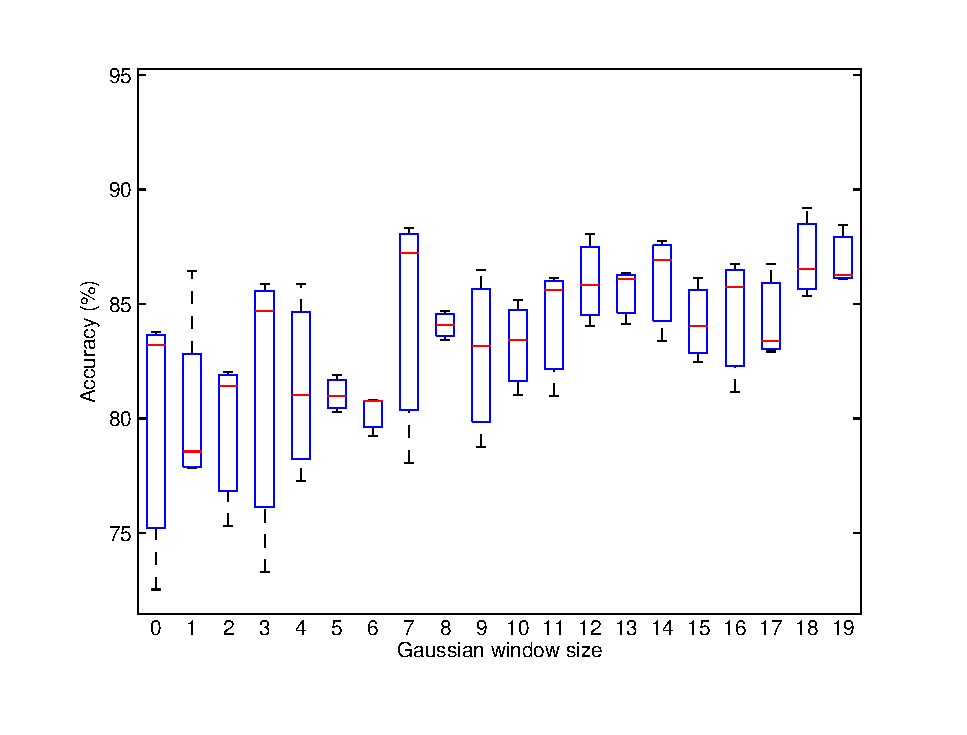
\includegraphics[height=2.3in,keepaspectratio]{./images/gaussian_window.eps}}\hspace{1em}%
  \subcaptionbox{After removing water absorbtion bands\label{fig3:gaussian smoothing:b}}{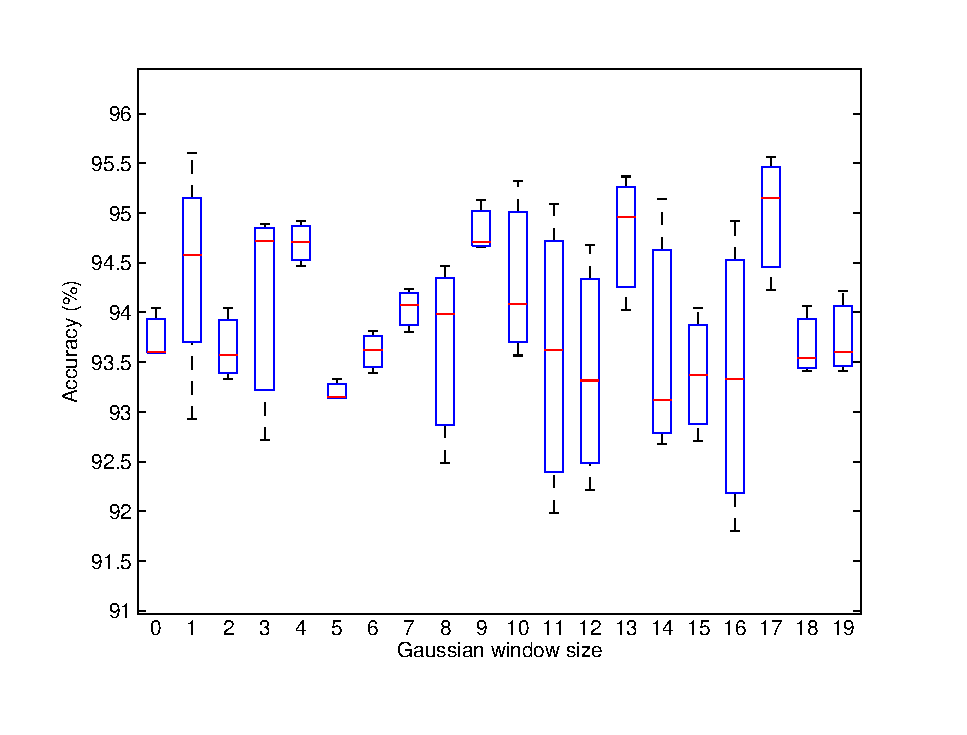
\includegraphics[height=2.3in,keepaspectratio]{./images/gaussian_window_filtered_water_absorbtion_bands.eps}}
   \caption{Effect of Gaussian smoothing window size on SVM accuracy using polynomial kernel degree 3}
 \label{fig:gaussian smoothing}
\end{figure}


\section{Results and Discussion}

Gaussian smoothing increases accuracy by about 10\% on raw data, but after preprocesings such as removing various water absorbtion bands its effects become marginal. We observe that after removing water absorbtion bands the we reach an accuracy of about 94\%. In general we suggest a Gaussian window of size 4 or 8 beyind that data although we might get slight changes in accuracy, but due to major structure changes, data loses its meaning. You can view the confusion matrix in Table \ref{table:confusion matrix}. 

For future work we can consider adding the following sections to paper: 

\begin{itemize}
\item Gaussian Smoothing OK
\item \red{compare atcor and flaash}
\item \red{Adding Lidar and classification using it}
\item \red{knowledge reasoning on enhancing mis-classification of Live oak vs Pine}
\item \red{other cassification methods and their comparison diagrams}
\item \red{parameter tuning for SVM charts}
\item \red{global predicted maps with legend}
\item \red{robustness Dr. Gader}

\item \red{Add endmember features and verify its utility in enhancing classification accuracy}
\item \red{Mention that the actual neon system will be at higher resolution}
\item \red{compare airborne reflectance to ground}

\end{itemize}






% http://tex.stackexchange.com/questions/42968/reduction-of-space-between-two-sub-figures
\begin{figure}[htp]
  % Fixed length
  \centering
  \subcaptionbox{Tuning polynomial order for SVM with polynomial kernel function\label{fig3:a}}{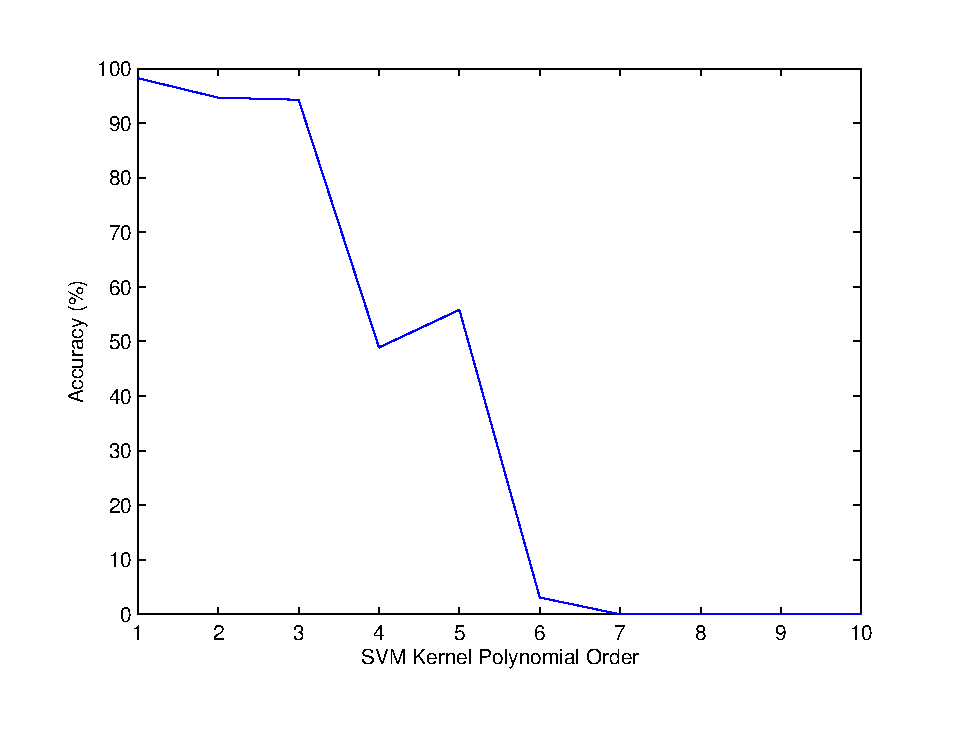
\includegraphics[height=2.1in,keepaspectratio]{./images/svm_kernel_polynomial_order.eps}}\hspace{1em}%
  \subcaptionbox{Tuning $\sigma$ in SVM with RBF kernel function\label{fig3:b}}{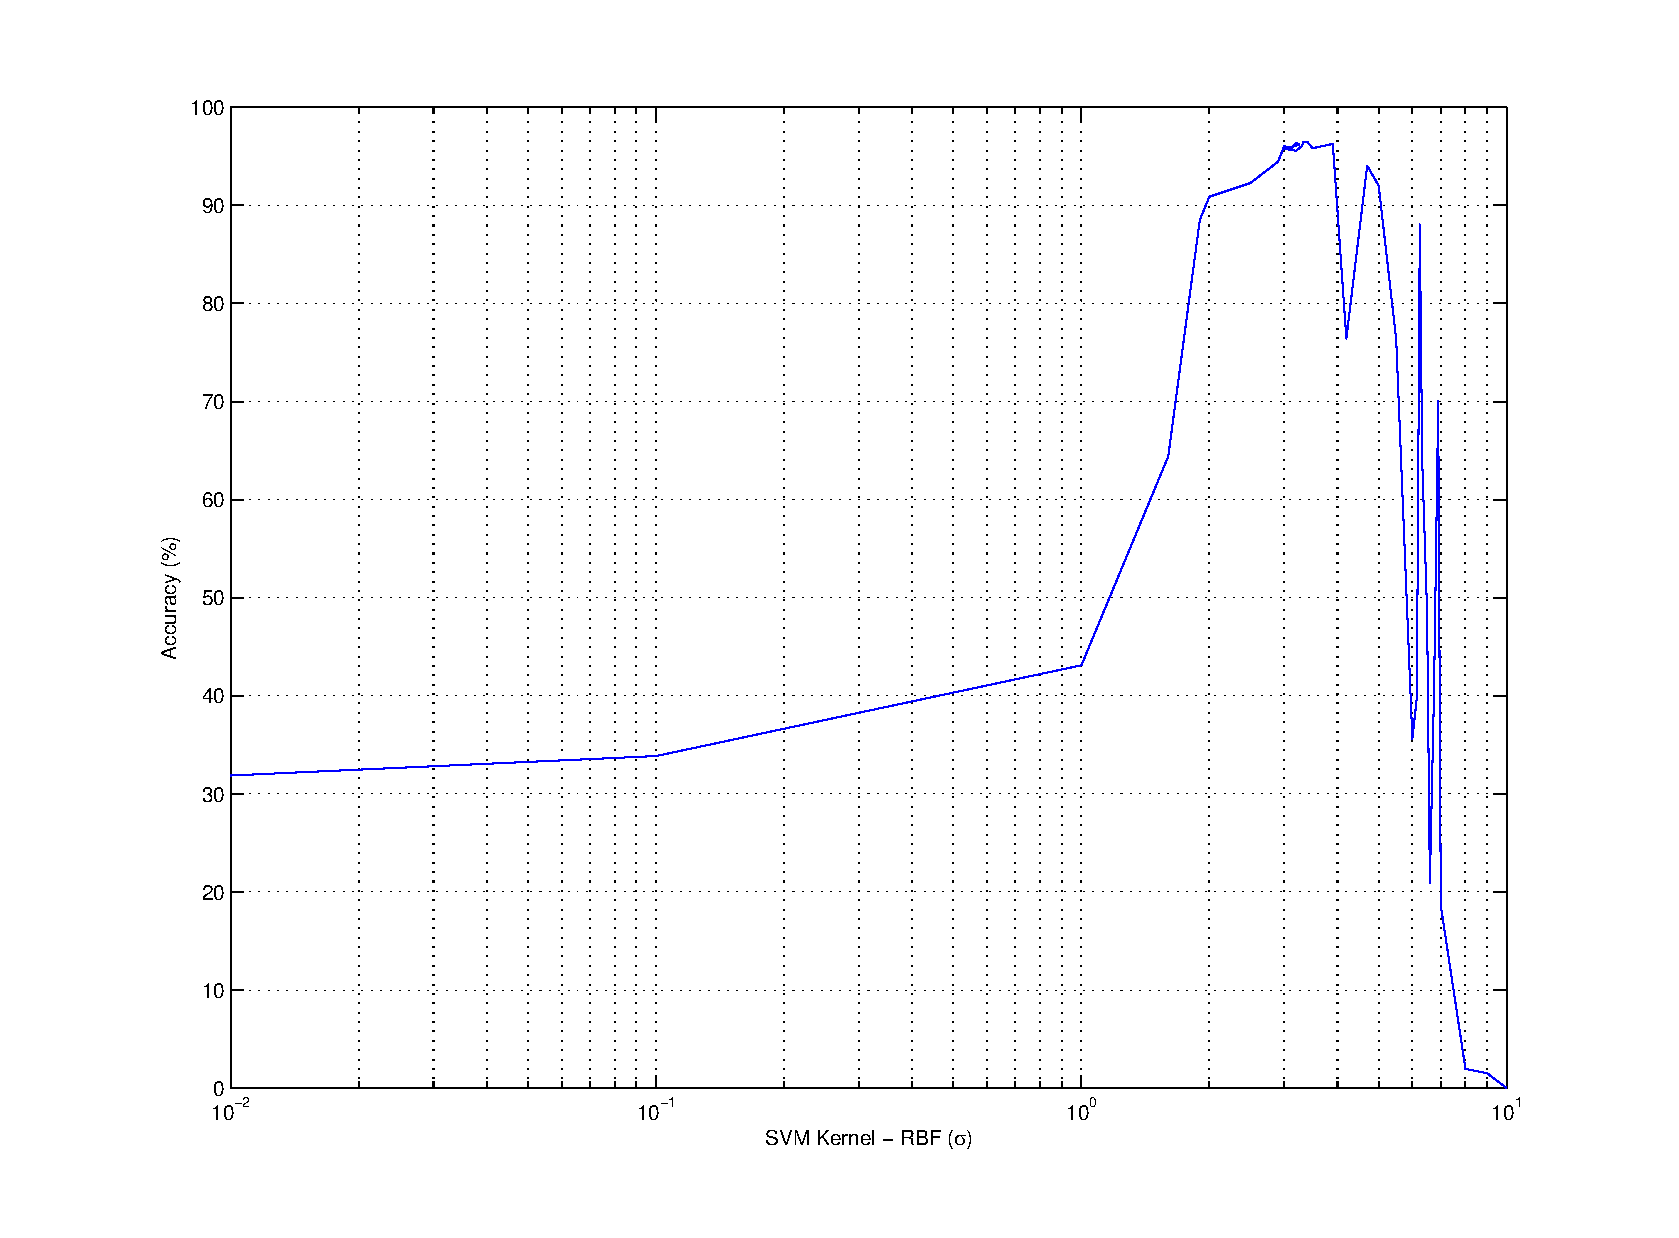
\includegraphics[height=2.1in,keepaspectratio]{./images/svm_kernel_rbf.eps}}
   \caption{Parameter tuning for classification algorithms}
       \label{fig:parameter tuning}

\end{figure}




%% Example of a theorem:
%\begin{Theorem}
%Text text text
%\end{Theorem}

%% Example of a proof:
%\begin{proof}[Proof of Theorem 1]
%Text text text
%\end{proof}


%%%%%%%%%%%%%%%%%%%%%%%%%%%%%%%%%%%%%%%%%%

\section{Conclusions}

Identifying species using remote sensing technologies such as hyperspectral and LiDAR sensors has a critical utility in studying global warming, bio-mass estimation, carbon preserves, invasive species identification and etc. NEON is about to begin as a thirty-year project at continental scale with goals on ecological monitoring one of which is remote sensing. In this paper we perform specie classification using SVM and the AVRIS hyperspectral and LiDAR data available via NEON. Our results show we have developed a promissing and robust classifier for determining tree species. 

%\acknowledgements{Acknowledgements}

%This work is supported ...

%%%%%%%%%%%%%%%%%%%%%%%%%%%%%%%%%%%%%%%%%%

% \authorcontributions{Author Contributions}

% Main text.

%%%%%%%%%%%%%%%%%%%%%%%%%%%%%%%%%%%%%%%%%%

%\conflictofinterests{Conflicts of Interest}

%State any potential conflicts of interest here or ``The authors declare no conflict of interest''. 

\bibliography{citation}
\bibliographystyle{mdpi}

\end{document}

